\documentclass[12pt,letterpaper]{article}

% Standard Overleaf packages; compile with pdfLaTeX.
\usepackage{iftex}
\ifPDFTeX
  \usepackage{cmap}
  \usepackage[T1]{fontenc}
  \usepackage[utf8]{inputenc}
  \usepackage{lmodern}
\else
  \usepackage{fontspec}
  \setmainfont{lmroman10-regular.otf}[
    BoldFont=lmroman10-bold.otf,
    ItalicFont=lmroman10-italic.otf,
    BoldItalicFont=lmroman10-bolditalic.otf]
\fi
\usepackage[margin=1in]{geometry}
\usepackage{amsmath,amssymb}
\usepackage{graphicx}
\usepackage[authoryear,round,sort]{natbib}
\setcitestyle{aysep={,},citesep={;}}
\usepackage[hidelinks]{hyperref}

% Plain, single-column text, without running headers or line numbers.
\pagestyle{plain}
\setlength{\parindent}{0pt}
\setlength{\parskip}{0.6em}
\setlength{\emergencystretch}{3em}
\linespread{1.08}
\urlstyle{same}

\begin{document}
\raggedright

\begin{center}

{\Large\bfseries Model-based inference of reward identity in the lateral orbitofrontal cortex\par}

\medskip

Qingfang Liu\textsuperscript{a}, Yao Zhao\textsuperscript{b}, Taaseen Khan\textsuperscript{c}, Nicole Moussa\textsuperscript{a}, Geoffrey Schoenbaum\textsuperscript{a}, Thorsten Kahnt\textsuperscript{a,1}\par

\medskip

\textsuperscript{a}National Institute on Drug Abuse Intramural Research Program, Baltimore, MD 21224, USA\par

\textsuperscript{b}Department of Psychology, University of Pennsylvania,
Philadelphia, PA 19104, USA\par

\textsuperscript{c}Feinberg School of Medicine, Northwestern University,
Chicago, IL 60611, USA\par

\end{center}


\section*{Abstract}
Flexible behavior requires using learned relationships to infer outcomes that have not been directly experienced. It remains unclear whether such inference retrieves only scalar value or the identity of a specific expected outcome. We combined sensory preconditioning, selective outcome devaluation, and functional MRI to test the content and neural representation of inferred outcomes in humans. Participants first learned associations between pairs of visual cues and then learned that the second cue of each pair predicted a specific food odor. After selective satiation devalued one of the food odors, choices decreased not only for cues directly associated with that odor but also for preconditioned cues whose outcomes had to be inferred through the associative structure. This transfer of devaluation indicates that model-based inference recovers the specific identity of outcomes rather than their cached value. Importantly, multivariate analysis of fMRI responses to preconditioned cues revealed inferred outcome-identity representations in the lateral orbitofrontal cortex (OFC). Moreover, representations of inferred outcome identity in lateral OFC were shared with those evoked by experienced outcomes. In contrast, these representations were not significant for conditioned cues. To account for this pattern, we propose a resource-limited framework in which outcome expectations receive greater representational resources when they provide greater computational benefit. Together, these findings show that human model-based inference accesses specific reward identities and suggest that lateral OFC may prioritize outcome information according to its computational utility.


\section*{Significance statement}
Adaptive decisions often require inferring the consequences of choices that have never been directly experienced. Here, we show that such inference can recover the identity of a specific expected reward, not merely whether an outcome is good or bad. We further find that the lateral orbitofrontal cortex preferentially represents expected reward identity when it must be inferred through learned associations rather than recalled from direct experience. These findings suggest that the brain does not represent all outcome information equally but instead prioritizes detailed information when it is most useful for guiding behavior.


\noindent\textbf{Keywords:} goal-directed behavior $|$ cognitive map $|$ orbitofrontal cortex $|$ outcome-guided behavior $|$ resource-limited model


\noindent\textbf{Correspondence:} \textsuperscript{1}To whom correspondence should be addressed. E-mail: thorsten.kahnt@nih.gov


\noindent\textbf{Author contributions:} Q.L., Y.Z., G.S., and T. Kahnt designed research; Q.L., Y.Z., T. Khan, and N.M. performed research; Q.L. and T. Kahnt analyzed data; Q.L. developed the theoretical model; G.S. and T. Kahnt supervised research; Q.L. wrote the original draft; and all authors reviewed and edited the manuscript.


\noindent\textbf{Competing interests:} The authors declare no competing interest.

\section*{Introduction}

Model-based behavior requires mental simulation of outcomes that have never been
directly experienced \citep{daw2011model,doll2015model,wangkahnt21}. Rather than relying only on cached values learned through direct reinforcement, animals can infer the likely consequences of a choice by combining separately learned associations. Such model-based inference supports adaptive behavior, while impairments in this process may contribute to maladaptive or compulsive behavior, including substance use disorders \citep{kahsch21,kahnt2023computationally}.

Sensory preconditioning (SPC) provides a behavioral framework for studying such inference \citep{kahnt2023computationally,jones12,wang2020interactions}. In a typical SPC procedure, neutral cue pairs are first learned (A $\rightarrow$ B, C $\rightarrow$ D), after which the second cue from each pair is directly conditioned with an outcome (B $\rightarrow$ reward, D $\rightarrow$ no reward). During a subsequent probe test without feedback, responding to cue A over C indicates that subjects have inferred the outcome associated with cue B from the learned A--B and B--reward associations.

Prior work indicates that the orbitofrontal cortex (OFC) is necessary for responding to preconditioned but not directly conditioned cues during the probe phase. For example, inactivating the OFC in rats during the probe test leaves responding to cue B, which was directly associated with reward, intact, while selectively impairing responding to cue A, which requires inferring the associated reward \citep{jones12}. Consistent findings have been observed in humans: targeting the OFC network with transcranial magnetic stimulation (TMS) before the probe test of the SPC task selectively disrupted inference-based responding to cue A without affecting responding to cue B \citep{wang2020targeted}.  Together, these results provide cross-species evidence for a role of the OFC in model-based inference.

However, it remains unclear what information is inferred during SPC. In particular, behavioral responses to preconditioned cues could reflect inference of either the scalar value or the specific identity of the reward associated with conditioned cues. The former possibility is that SPC supports inference over reward value: a cue may come to predict that ``something good'' or ``something bad'' will occur. The latter possibility is that subjects infer a specific reward: a cue may predict a specific outcome, such as a particular food odor, whose value can later be updated. Given extensive evidence that OFC represents reward identity \citep{klein2013segregated,mcnamee13,RN14,howard2015identity,howard2017identity,howard2018identity,howard2021specific,liuyaoatt24,witkowski2026identity}, this possibility raises a further question: does lateral OFC represent inferred and directly learned outcome identities in the same manner?


Selective outcome devaluation provides a direct test of the question whether cached value or outcome identity is expected \citep{HowRey2020,liu2025distinct,hart20}. In this procedure, after learning an association between a cue and a specific reward, the value of that reward is reduced through selective satiation or conditioned taste aversion. If responding to the cue depends on the expectation of a specific outcome, devaluing that outcome should reduce responding to cues that predict it. In contrast, if responding is driven by a cached scalar value that is not linked to the specific outcome identity, devaluing the outcome should have little or no effect on responding to the cue.




In the current work, we combined sensory preconditioning \citep{Brogden39} with outcome devaluation \citep{HowRey2020,liu2025distinct} to assess if inferred cue-outcome pairings are sensitive to devaluation. Participants learned associations between pairs of visual cues as well as between the second cues of each pair and one of two food odors before completing two probe tests, with a selective satiation procedure between the two probe tests to reduce the pleasantness of one of the food odors. Behaviorally, we asked whether devaluation changes choices for both directly conditioned and preconditioned cues, and whether these changes track individual changes in odor pleasantness. Neurally, we tested whether cue-evoked activity patterns in the OFC reflect outcome value or identity. We found, first, that devaluation altered choices for both directly conditioned and preconditioned cues, indicating that inference involves specific outcome identity rather than only cached value. Second, pattern-based fMRI analyses revealed that lateral OFC preferentially represented reward identity for preconditioned compared to conditioned cues. We propose a resource-limited framework model to account for the preferential representation of inferred outcomes in lateral OFC.






\par\bigskip\begingroup
\refstepcounter{figure}


\begin{center}
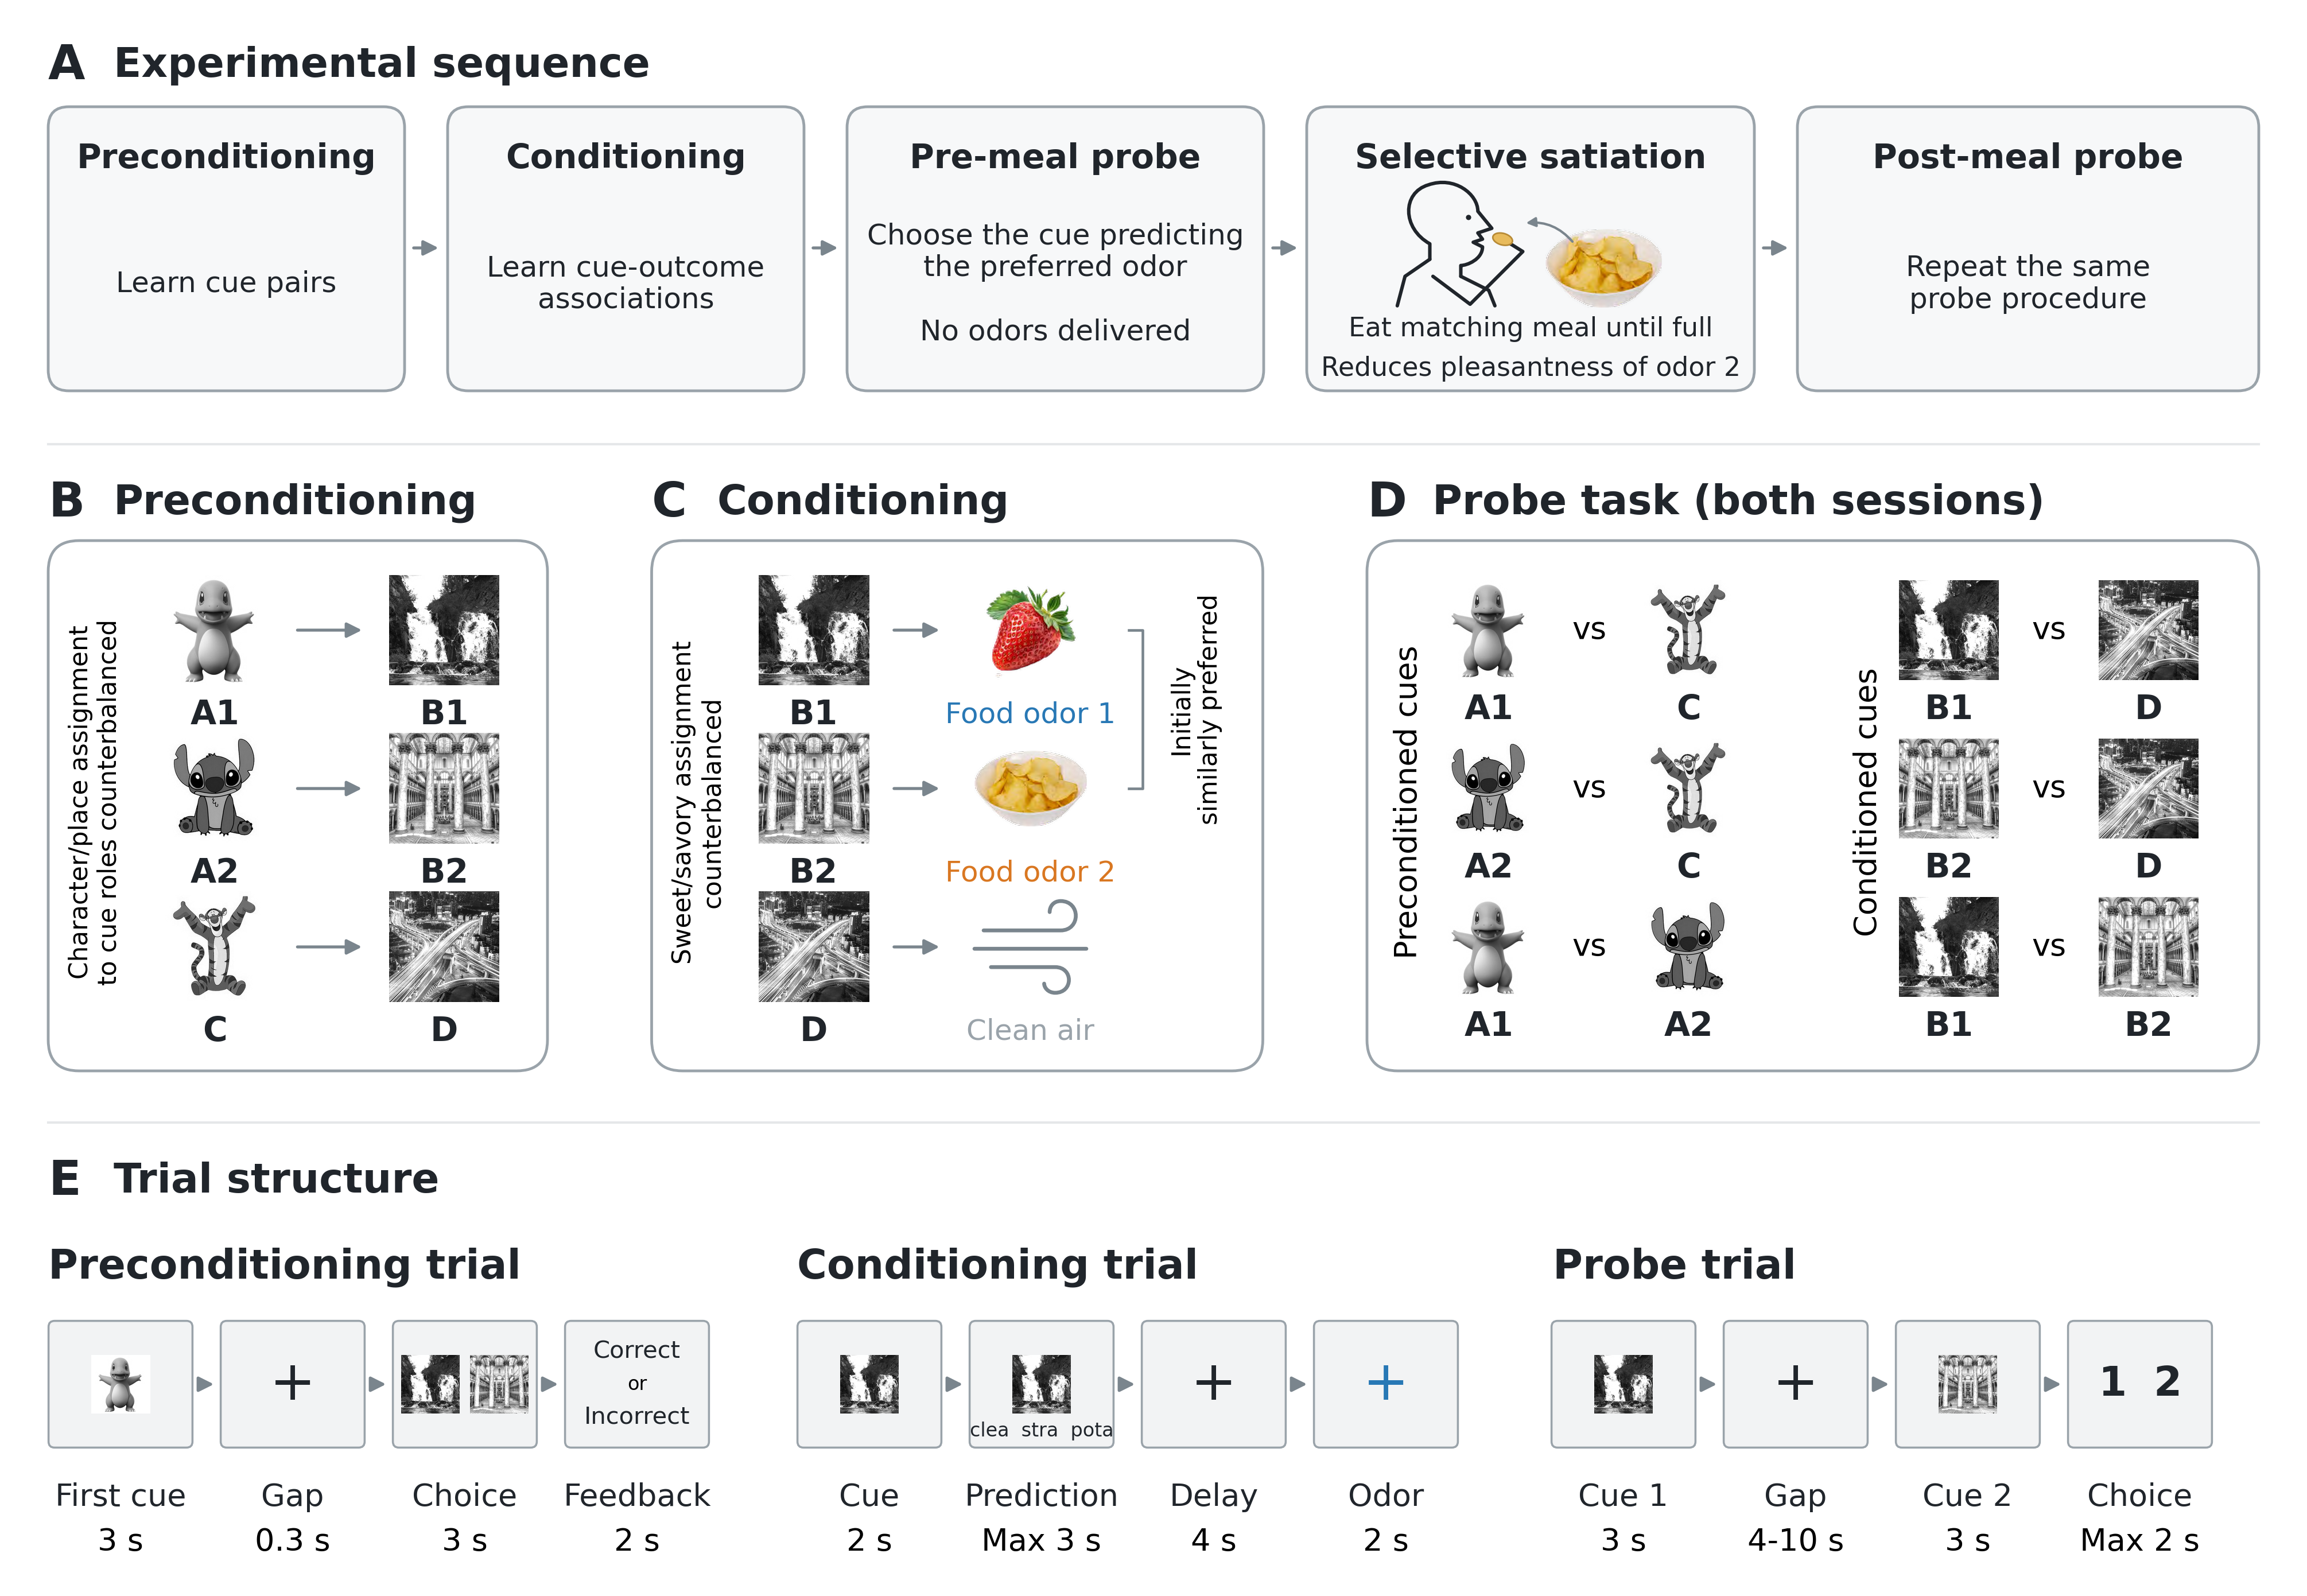
\includegraphics[width=0.95\linewidth]{../../fig/fig1_design.png}
\end{center}
\par\noindent\textbf{Figure~\thefigure. }\textbf{Experimental design.}
\textbf{A. Experimental sequence.} Preconditioning and conditioning were followed by a pre-meal probe, selective satiation, and a post-meal probe. During satiation, participants ate a meal matching food odor 2 until very full, reducing that odor's pleasantness. No odors were delivered during either probe session.
\textbf{B. Preconditioning.} Participants learned visual cue pairs: A1--B1, A2--B2, and C--D. The first cue served as the preconditioned cue (A1, A2, C), and the second as the conditioned cue (B1, B2, D). Character/place assignment to these cue roles was counterbalanced across participants.
\textbf{C. Conditioning.} B1 and B2 predicted two initially similarly preferred food odors (one sweet, one savory), labeled food odors 1 and 2; D predicted clean air. Food odor 2 was devalued only after the pre-meal probe. Sweet/savory assignment was counterbalanced; food images illustrate an example mapping.
\textbf{D. Probe task.} The same pairwise comparisons were presented before and after the meal, separately for preconditioned and conditioned cues. Participants chose the cue predicting their preferred odor or clean air.
\textbf{E. Trial structure.} During preconditioning, the first cue appeared for 3\,s, followed by a 0.3\,s gap and a 3\,s choice display containing the correct associate and one alternative from the same cue set. Participants responded via left/right keypress. Correct/incorrect feedback lasted 2\,s within the jittered 3--8\,s inter-trial interval, followed by fixation for the remainder. During conditioning, a cue appeared for 2\,s and remained visible during a prediction period of up to 3\,s, alongside three abbreviated odor names. After a 4\,s effective delay to odor arrival, the associated odor or clean air was delivered for 2\,s, followed by a jittered 4--10\,s inter-trial interval. During each probe trial, cue\,1 appeared for 3\,s, followed by a jittered 4--10\,s gap and cue\,2 for 3\,s. Participants then had up to 2\,s to choose, followed by a jittered 4--10\,s inter-trial interval. Display widths are schematic and do not encode duration.
\par

\label{fig-design}

\par\endgroup\bigskip





\section*{Results}
\label{sec-res}


\subsection*{Experimental design}
\label{subsec-design}



The experimental sequence is shown in \autoref{fig-design}A. During preconditioning (\autoref{fig-design}B), participants learned associations between pairs of visual cues. We refer to the first cue in a pair as the preconditioned cue (A1, A2, C) and the second cue as the conditioned cue (B1, B2, D). Next, during conditioning (\autoref{fig-design}C), participants learned associations between conditioned cues and two specific food odor rewards (one savory, one sweet, equally preferred) as well as clean air. This was followed by pre-meal and post-meal probe tests (\autoref{fig-design}D), in which preferences for all cues were assessed. The two probe test sessions were separated by a devaluation procedure, in which participants consumed a meal matching the food odor predicted by B2. The meal-matched and non-matched odors are referred to as the devalued and non-devalued odors, respectively. Trial timing is shown in \autoref{fig-design}E.

Previous work has shown that consuming a meal matching a food odor selectively devalues this food odor but leaves the value of non-matched food odors intact \citep{howard2017identity,HowRey2020,liu2025distinct}. This leads to a change in preference from the pre- to the post-meal probe test, such that after the meal, participants prefer conditioned cues associated with the non-devalued food odor over cues associated with the devalued food odor \citep{HowRey2020,liu2025distinct}. However, it is unknown whether this devaluation also transfers to the preconditioned cues. Answering this question gives insights into the content of the inference. If preferences for preconditioned cues changed in the same way as for conditioned cues, this would indicate that inference acts on specific outcomes. In contrast, if there is no change in preferences, this would indicate that participants infer the cached reward value that they previously learned for conditioned cues.




\subsection*{Devaluation reduces choices for conditioned and preconditioned cues}
\label{subsec-beh}


Participants showed a clear learning pattern across runs during preconditioning (\autoref{fig-beh}A), with accuracy increasing from the initial training ($0.81 \pm 0.11$) to the final run ($0.99 \pm 0.03$; mean $\pm$ SD). Accuracy did not differ across the three cue pairs (A1--B1, A2--B2, and C--D; Friedman test: $\chi^2(2) = 0.29$, $p = 0.867$). During conditioning (\autoref{fig-beh}B), accuracy of odor predictions also improved steadily across runs. By the final run, all participants reached at least 0.75 accuracy (mean $\pm$ SD $= 0.94 \pm 0.069$), and final accuracy did not differ among cues B1, B2, and D (Friedman test: $\chi^2(2) = 3.887$, $p = 0.143$).


We confirmed the effectiveness of our selective satiation procedure by analyzing changes in odor pleasantness ratings from before to after the meal (\autoref{fig-beh}C). The devalued odor showed a significant decrease in pleasantness following the meal ($W = 30.0$, $p < 0.001$; Wilcoxon signed-rank test), whereas pleasantness ratings for the non-devalued odor did not change significantly ($W = 127.5$, $p = 0.139$). The pre-to-post decrease was significantly greater for the devalued than the non-devalued odor ($W = 78.0$, $p = 0.0013$; one-sided Wilcoxon signed-rank test), consistent with a sensory-specific satiety effect. There was also no significant change in pleasantness ratings for clean air ($W = 54.0$, $p = 0.286$).


Importantly, in line with previous work \citep{HowRey2020,liu2025distinct}, this selective devaluation affected choices during the probe test. Choice proportions for conditioned cues associated with the devalued food odor (B2) decreased after the meal, both in the $B2>B1$ ($W = 27.0$, $p = 0.0021$) and $B2>D$ choice pairs ($W = 31.0$, $p = 0.0168$; two-sided Wilcoxon signed-rank tests; \autoref{fig-beh}D). Choices for the conditioned cue associated with the non-devalued food odor showed no significant change from pre- to post-meal ($B1>D$: $W = 97.5$, $p = 0.5309$; two-sided Wilcoxon signed-rank test). The pre-to-post decrease was numerically greater for $B2>D$ than for $B1>D$, but this difference was not significant ($W = 68.5$, $p = 0.0511$; one-sided Wilcoxon signed-rank test).

Critically, we observed a similar pattern for preconditioned cues that were indirectly associated with the devalued food odor (A2), such that participants were less likely to select A2 in both the $A2>A1$ ($W = 27.0$, $p = 0.0021$) and $A2>C$ choice pairs ($W = 23.5$, $p = 0.0069$; \autoref{fig-beh}E), with no significant change from pre- to post-meal for $A1>C$ ($W = 70.5$, $p = 0.1972$; all two-sided Wilcoxon signed-rank tests). The pre-to-post decrease was numerically greater for $A2>C$ than for $A1>C$, but this difference was not significant ($W = 138.0$, $p = 0.1102$; one-sided Wilcoxon signed-rank test). These results are consistent with devaluation transfer to preconditioned cues and access to specific outcome information.




\par\bigskip\begingroup
\refstepcounter{figure}


\begin{center}
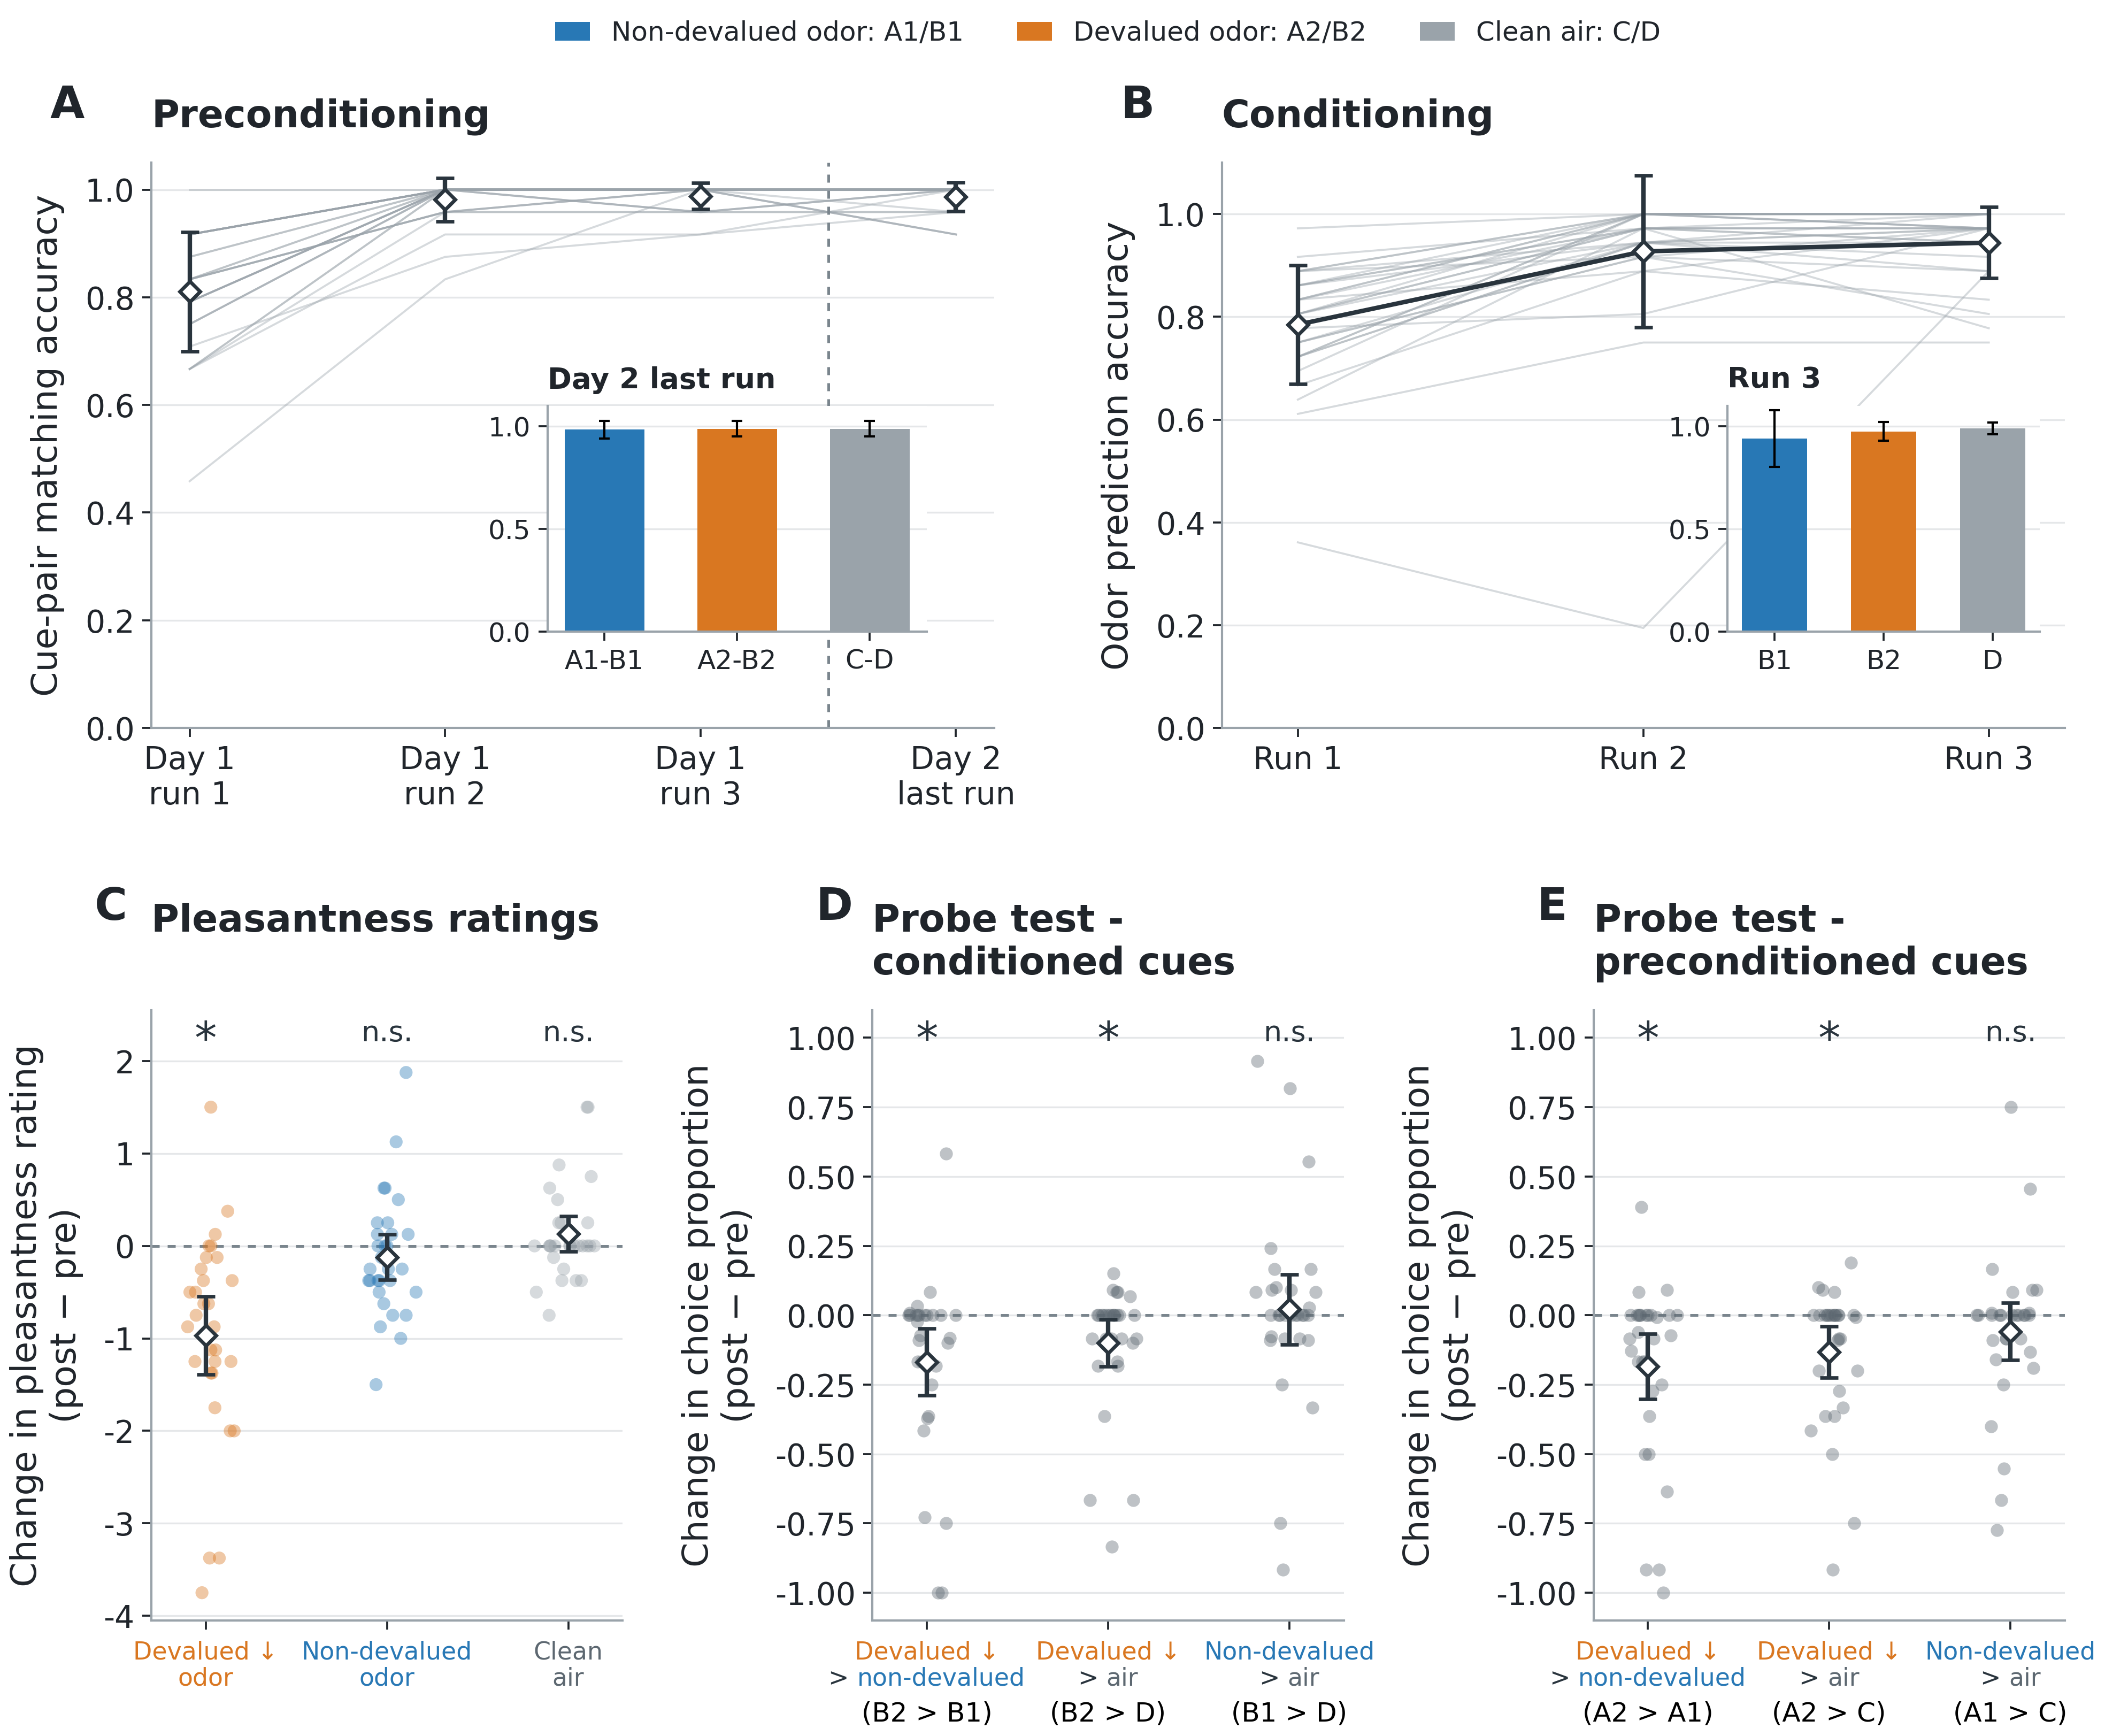
\includegraphics[width=0.95\linewidth]{../../fig/fig2_behavior.png}
\end{center}
\par\noindent\textbf{Figure~\thefigure. }
\textbf{Devaluation reduces choices for conditioned and preconditioned cues.}
\textbf{A. Preconditioning accuracy across runs.} Open diamonds indicate mean accuracy with standard-deviation bars; thin gray lines show individual participants. Inset shows mean accuracy with standard-deviation bars for the three pair types (A1--B1, A2--B2, C--D) in the final preconditioning run. Color denotes cue pairs later associated with non-devalued odor (blue), devalued odor (orange), and clean air (gray).
\textbf{B. Conditioning accuracy across runs.} Thin gray lines show individual participants; connected open diamonds indicate mean accuracy with standard-deviation bars across the three runs. Inset shows mean accuracy with standard-deviation bars for B1, B2, and D in the final conditioning run. Color code as in A.
\textbf{C. Odor pleasantness changes from pre- to post-meal.} Negative values indicate reduced pleasantness after the meal. Pleasantness ratings decrease more for meal-matched than non-matched odors.
\textbf{D. Probe test - conditioned cues.} Choice proportion is defined as selecting the cue listed first over the cue listed second in a pair (e.g., $B2>B1$). The y-axis shows the post-meal minus pre-meal change in this proportion with negative values indicating reduced preference for the first cue named in each comparison. Dots represent individual participants, open diamonds indicate means, and error bars show t-based 95\% confidence intervals.
\textbf{E. Probe test - preconditioned cues.} Data as in D but for preconditioned cues. In C--E, label colors identify devalued odor (orange), non-devalued odor (blue), and clean air (gray); orange downward arrows denote predicted decreases following devaluation. All analyses include 31 participants, except for pleasantness ratings (30 participants because one participant's ratings were unavailable). Asterisks denote uncorrected $p < 0.05$ from two-sided Wilcoxon signed-rank tests of paired changes against zero; n.s., not significant.
\par

\label{fig-beh}

\par\endgroup\bigskip




\subsection*{Lateral OFC represents inferred reward identity}


Our behavioral findings indicate that participants inferred specific outcome identities from preconditioned cues. We next asked where these inferred outcome identities are represented in the brain. Given previous evidence that OFC responses to reward-predictive cues contain information about the identity of expected outcomes \citep{howard2015identity,howard2017identity,klein2013segregated,RN650,mcnamee2015associative,RN636,witkowski2026identity}, we tested whether preconditioned cues also evoke representations of their inferred food odors in the OFC.

We used representational similarity analysis (RSA) to test whether cues predicting the same food odor elicited more similar neural activity patterns than cues predicting different outcomes (\autoref{fig-rsa}B). We ran this analysis in independently defined regions of lateral and medial OFC (\autoref{fig-rsa}A) \citep{kahnt2012connectivity}. We separately analyzed fMRI responses to conditioned and preconditioned cues from trials of the pre-meal probe test, excluding cues associated with clean air. Neural pattern comparisons were restricted to cue presentations from different runs, and we only used data from the first cue in each trial. Neural patterns evoked by preconditioned cues reflected the identities of their indirectly associated food odors in lateral OFC (mean Spearman $\rho = 0.029$, $t(30) = 2.35$, $p = 0.013$), whereas this effect was not significant in medial OFC (mean Spearman $\rho = 0.013$, $t(30) = 0.91$, $p = 0.186$; \autoref{fig-rsa}C). In contrast and unexpectedly, parallel analyses for the conditioned cues were not significant in either area (all $p > 0.05$; \autoref{fig-rsa}C).


\par\bigskip\begingroup
\refstepcounter{figure}


\begin{center}
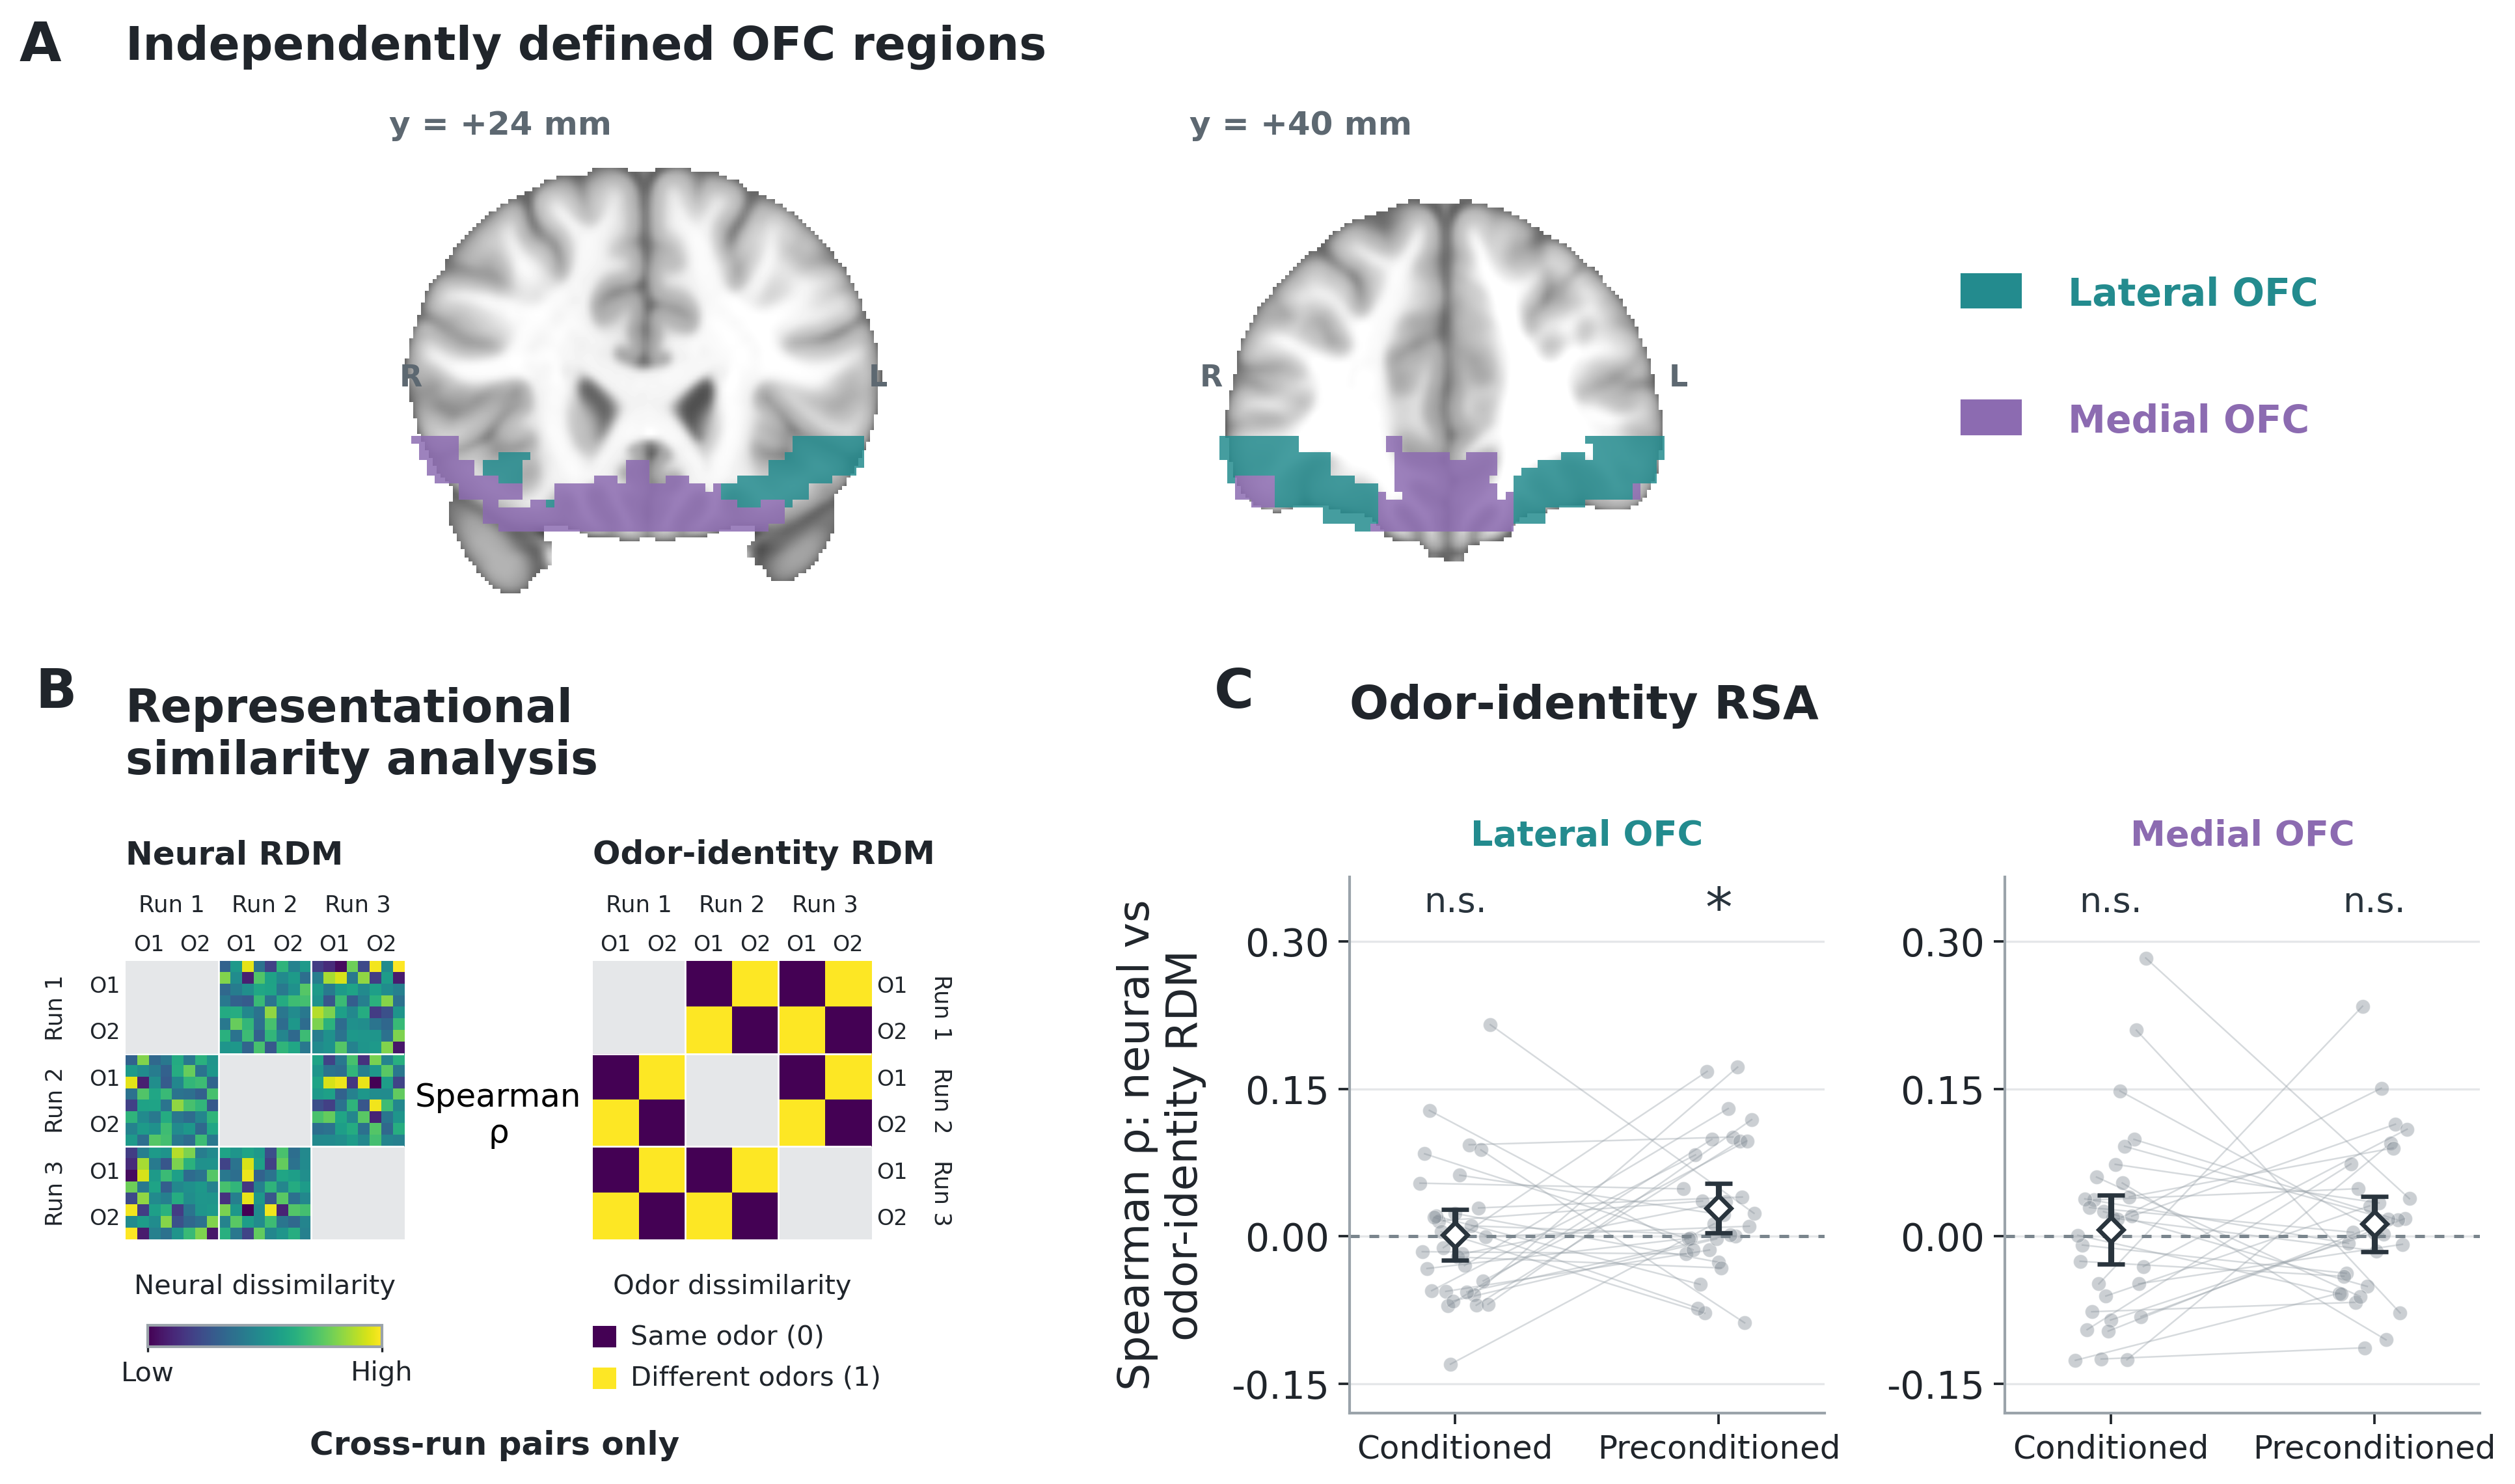
\includegraphics[width=0.95\linewidth]{../../fig/fig3_rsa.png}
\end{center}
\par\noindent\textbf{Figure~\thefigure. }
\textbf{Lateral OFC represents inferred reward identity.}
\textbf{A. Independently defined OFC regions.} Coronal views at MNI $y = 24$ and $40$\,mm show the bilateral connectivity-based OFC regions. Short labels are used throughout the text and figure: lateral OFC (teal) denotes central/anterior-lateral OFC, and medial OFC (purple) denotes medial/posterior-lateral OFC. Anatomical right is shown on the left.
\textbf{B. Representational similarity analysis.} Neural representational dissimilarity matrices (RDMs; one minus the Pearson correlation between activity patterns) were compared with an odor-identity RDM assigning zero dissimilarity to cues predicting the same odor and unit dissimilarity to cues predicting different odors. Matrices illustrate first-cue pre-meal responses to preconditioned odor-predictive cues in lateral OFC from the first retained participant (sub-01), with presentations ordered by run and odor identity. Neural dissimilarities range from 0.51 to 1.47 in this example. Gray blocks mark within-run comparisons, which were excluded. Spearman correlations were calculated using unique cross-run pairs, separately for conditioned and preconditioned cues. Clean-air-associated cues were excluded.
\textbf{C. Odor-identity RSA results.} Participant-level correlations between neural and odor-identity RDMs are shown for each cue type and ROI. Dashed lines indicate zero correlation. In C, points represent individual participants ($n = 31$), gray lines connect measurements from the same participant, and open diamonds indicate means with t-based 95\% confidence intervals. Asterisks denote uncorrected $p < 0.05$ from one-sided one-sample $t$-tests against zero; n.s., not significant.
\par

\label{fig-rsa}

\par\endgroup\bigskip


\subsection*{Preconditioned cues reinstate representations of experienced rewards in lateral OFC}

The results reported above suggest that lateral OFC represents the identities of inferred outcomes. We next asked in what coding format inferred reward expectations are represented in lateral OFC. Previous work in monkeys has shown OFC responses during both reward expectation and receipt \citep{tremblay1999relative}. In humans, multivariate fMRI studies have shown shared value representations for expected and received rewards in OFC \citep{RN1,kahnt2011decoding}. Based on these findings, we tested the hypothesis that inferred reward identity representations are shared with those evoked when experiencing the reward, i.e., smelling the food odors.

To test this, we leveraged a cross-task decoding approach, using fMRI data from an independent localizer task (conducted before the main SPC task), in which subjects smelled each of the food odors. We trained a classifier to distinguish odor identities from neural responses from the localizer and tested it on cue-evoked responses during the pre-meal probe test (\autoref{fig-decoding}A). This cross-decoder successfully classified the expected odor identities in response to preconditioned cues in lateral OFC (decoding accuracy = 54.10\%; chance = 50\%; $t(30) = 2.22$, $p = 0.017$; \autoref{fig-decoding}B). We also examined cross-task decoding in medial OFC and for conditioned cues for comparison, although the preceding RSA did not provide significant evidence for reward-identity representations in these cases. Consistent with this pattern, cross-decoding was not significantly above chance for preconditioned cues in medial OFC or for conditioned cues in either region (all $p > 0.05$; \autoref{fig-decoding}B).

The cross-task decoding result in lateral OFC supports the interpretation that preconditioned cues reinstate a specific neural representation of the experienced food odor.




\par\bigskip\begingroup
\refstepcounter{figure}


\begin{center}
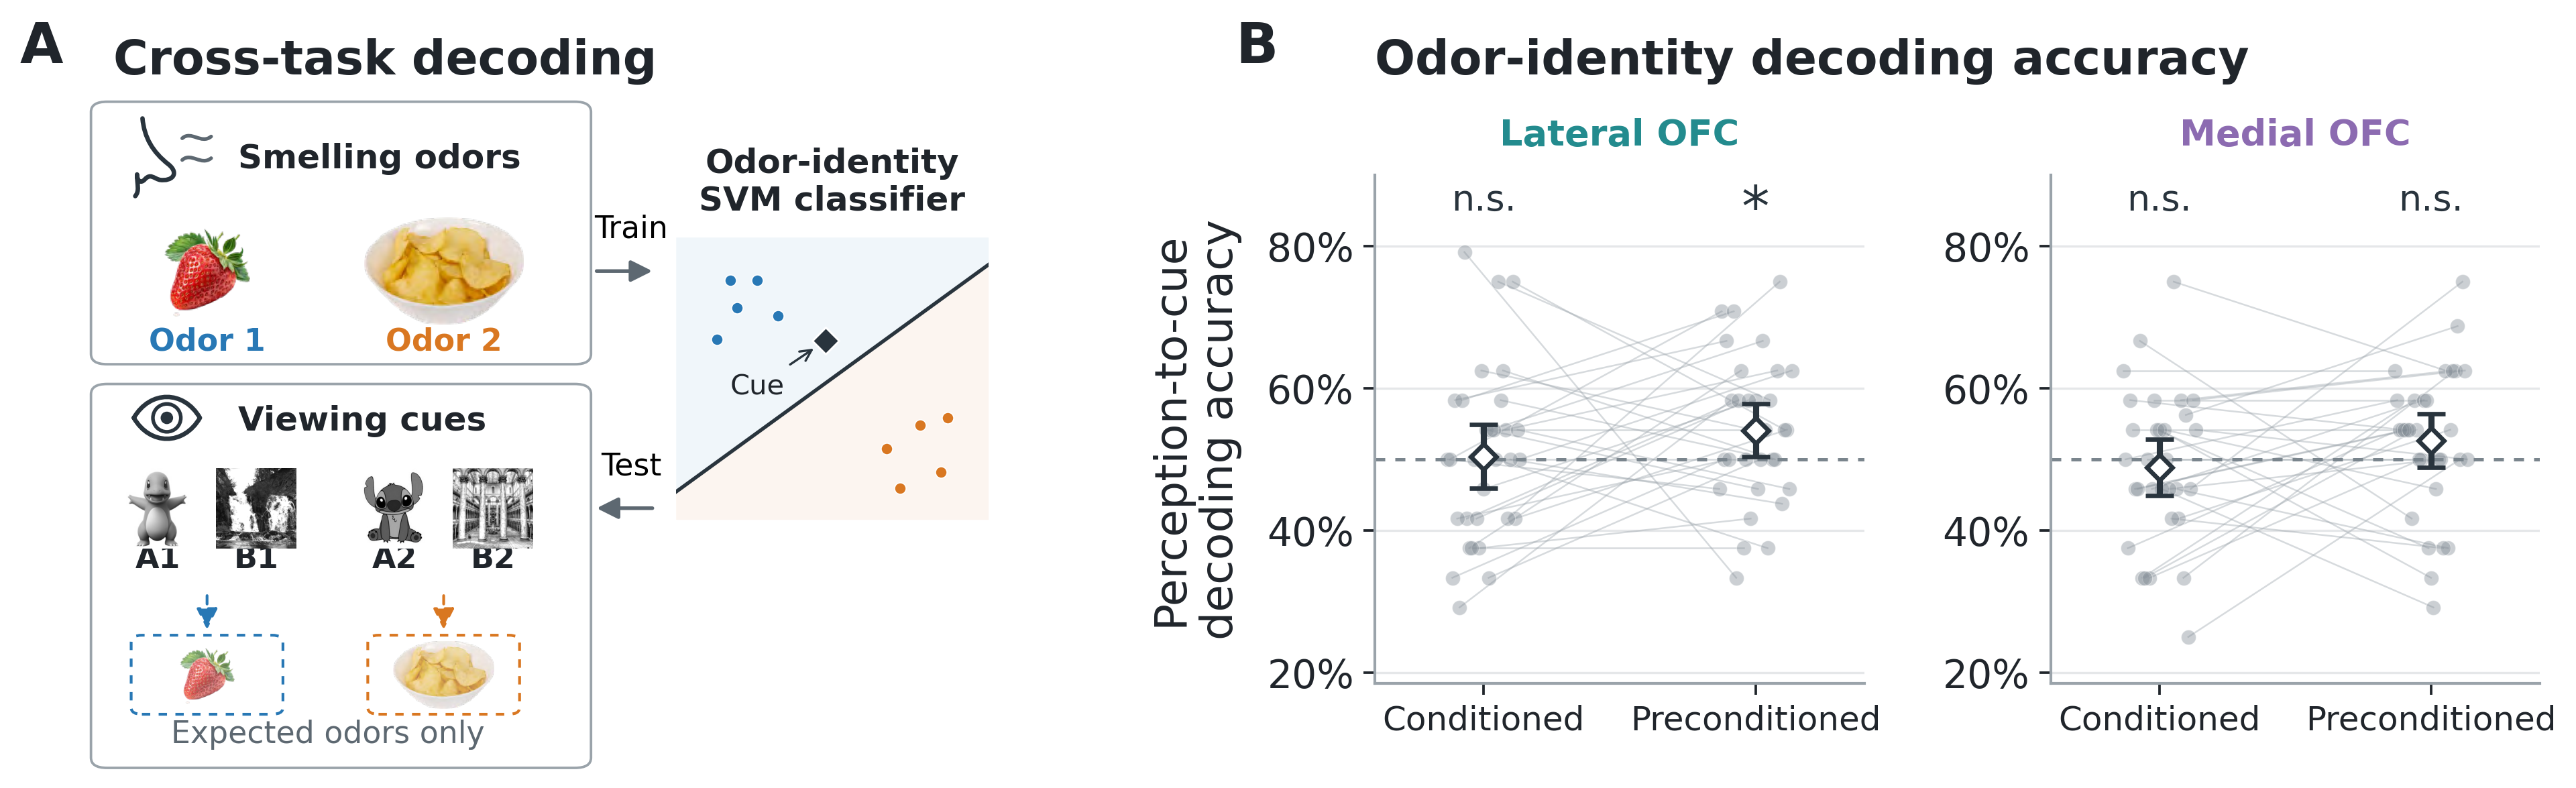
\includegraphics[width=0.95\linewidth]{../../fig/fig4_decoding.png}
\end{center}
\par\noindent\textbf{Figure~\thefigure. }
\textbf{Preconditioned cues reinstate representations of experienced rewards in lateral OFC.}
\textbf{A. Cross-task decoding.} A linear support vector machine (SVM) was trained to distinguish neural responses to two passively presented odors and tested on responses to the first cue of each pre-meal probe trial, during which no odors were delivered. Odor symbols and cue images follow the illustrative mapping in \autoref{fig-design}. Solid boxes separate training and testing; dashed arrows link cues to their expected odors, shown in dashed boxes to indicate that they were not delivered during testing. The decision boundary, training patterns, and cue pattern illustrate classification in schematic neural pattern space and do not depict measured two-dimensional data. Conditioned and preconditioned odor-predictive cues were evaluated separately; clean-air-associated cues were excluded.
\textbf{B. Odor-identity decoding accuracy.} Decoding accuracy measures generalization from odor perception to odor expectation. Dashed lines indicate chance accuracy (50\%). In B, points represent individual participants ($n = 31$), gray lines connect measurements from the same participant, and open diamonds indicate means with t-based 95\% confidence intervals. Asterisks denote uncorrected $p < 0.05$ from one-sided one-sample $t$-tests against chance; n.s., not significant.
\par

\label{fig-decoding}

\par\endgroup\bigskip





\subsection*{Value-related representations in medial OFC}

Beyond identifying the expected outcome, successful choice also depends on representing its current subjective value. Prior work has shown that activity in medial OFC signals the subjective value of outcomes \citep{bartra2013valuation}. In our task, probe test choices tracked participants' individual pleasantness ratings (Fig.~S4), and selective satiation altered the value of the meal-matched outcome between the two probe tests. We therefore asked whether cue-evoked fMRI patterns in OFC reflected expected outcome value.

To localize value-related representations, we performed a searchlight multiple-regression RSA combining data from the pre- and post-devaluation probe tests ($n = 30$). Analyses included conditioned and preconditioned cues associated with either food odor or clean air, and responses to both first and second cue presentations. After jointly standardizing each participant's odor pleasantness ratings across pre- and post-meal sessions, we assigned each cue presentation its associated outcome rating from the corresponding phase. The value RDM captured pairwise differences in outcome pleasantness. We tested whether larger value differences predicted greater fMRI pattern dissimilarity. Model fitting used only comparisons between different runs, including comparisons across probe phases (Supplementary Methods).

Neural dissimilarity increased with differences in expected outcome value in medial OFC ($t(29) = 4.42$, peak-level $p_{\mathrm{FWE}} = 0.032$, small-volume corrected; Fig.~S5). The corresponding effect did not survive correction in lateral OFC ($t(29) = 2.87$, $p_{\mathrm{FWE}} = 0.503$). These findings are consistent with previous evidence implicating medial OFC in representing subjective value \citep{levy2012root,mcnamee13,howard2015identity}.

\subsection*{A resource-limited model of outcome-identity representation}

To explain the unexpected preferential representation of outcome-specific expectations evoked by preconditioned over conditioned cues in lateral OFC, we propose a resource-limited account in which explicit outcome-identity representations are allocated according to their computational value (\autoref{fig-identity-simu}). For cue class $i \in \{P,C\}$, where $P$ and $C$ denote preconditioned and directly conditioned cues, respectively, we assume that decision loss decreases exponentially with the resource devoted to outcome-identity representation (\autoref{fig-identity-simu}A):


\begin{equation}
L_i = a_i e^{-r_i},
\end{equation}

where $r_i$ is the representational resource devoted to that cue's outcome identity, and $a_i$ captures the computational value of explicitly representing it. The exponential form captures diminishing returns: additional representational resources produce progressively smaller reductions in decision loss. We adopt this form as a simple, analytically tractable implementation of that assumption.

To illustrate computational value with an everyday analogy, consider shipping a fragile item: the value of preventing breakage is the probability that it breaks multiplied by the cost of replacing it. Similarly, the computational value of explicit identity representation depends on how likely outcome-identity retrieval is to fail and how costly that failure would be. We therefore define

\begin{equation}
a_i = q_i D_i,
\end{equation}

where $q_i$ is the baseline probability of failing to recover the correct outcome identity for cue $i$, and $D_i$ is the behavioral cost of that failure. $q_P$ and $q_C$ denote this baseline failure probability for preconditioned and conditioned cues, respectively. Conditioned cues were directly paired with their outcomes ($C \rightarrow O$), whereas preconditioned cues require combining separately learned associations ($P \rightarrow C \rightarrow O$). Each associative step can fail to retrieve the correct associate. Recovering the outcome identity through two associations therefore requires successful retrieval at both steps, introducing an additional opportunity for error compared with a single association. We consequently assume that outcome-identity retrieval errors are more likely for preconditioned than for conditioned cues ($q_P > q_C$). Assuming identical behavioral costs of an identity error across cue types ($D_P = D_C$), this difference in failure probability implies $a_P > a_C$.

When preconditioned and directly conditioned cue classes share a fixed representational budget,
$r_P + r_C = R$, total loss is

\begin{equation}
L = a_P e^{-r_P} + a_C e^{-r_C}.
\end{equation}

At an interior optimum, the marginal benefit of assigning additional resource to the preconditioned cue equals the marginal cost of removing that resource from the conditioned cue (\autoref{fig-identity-simu}B; see Supplementary Methods for the derivation),

\begin{equation}
a_P e^{-r_P} = a_C e^{-r_C}.
\end{equation}

Therefore, under these assumptions, representing expected outcomes has greater computational value for preconditioned cues ($a_P > a_C$), and the optimal solution assigns more resources to their outcome identities ($r_P > r_C$; \autoref{fig-identity-simu}C). Thus, under this model, preferential representation of outcomes associated with preconditioned cues emerges from differences in computational utility, consistent with the pattern observed in lateral OFC (\autoref{fig-rsa}C and \autoref{fig-decoding}B).

The shared resource budget makes a further, testable prediction: within each participant, allocating more resources to directly associated outcomes leaves fewer resources for inferred outcomes. Holding total capacity constant and imposing $a_P>a_C$ for all 100 simulated participants, simulations illustrated this trade-off as a negative correlation between the two representations (Spearman $\rho = -0.324$; \autoref{fig-identity-simu}D; see Supplementary Methods for the sampling procedure).

To test whether this trade-off was also present in our data, we correlated odor-identity RSA coefficients for conditioned and preconditioned cues across participants, separately within each OFC region. Consistent with the predicted competition, these coefficients were negatively correlated in lateral OFC (Spearman $\rho = -0.317$, $p = 0.041$; one-sided test; \autoref{fig-identity-simu}E) but not in medial OFC (Spearman $\rho = -0.030$, $p = 0.437$).

Together, this resource-limited account explains how allocating representational resources according to computational value can produce both preferential representation of inferred outcome identities and competition between directly associated and inferred representations.




\par\bigskip\begingroup
\refstepcounter{figure}


\begin{center}
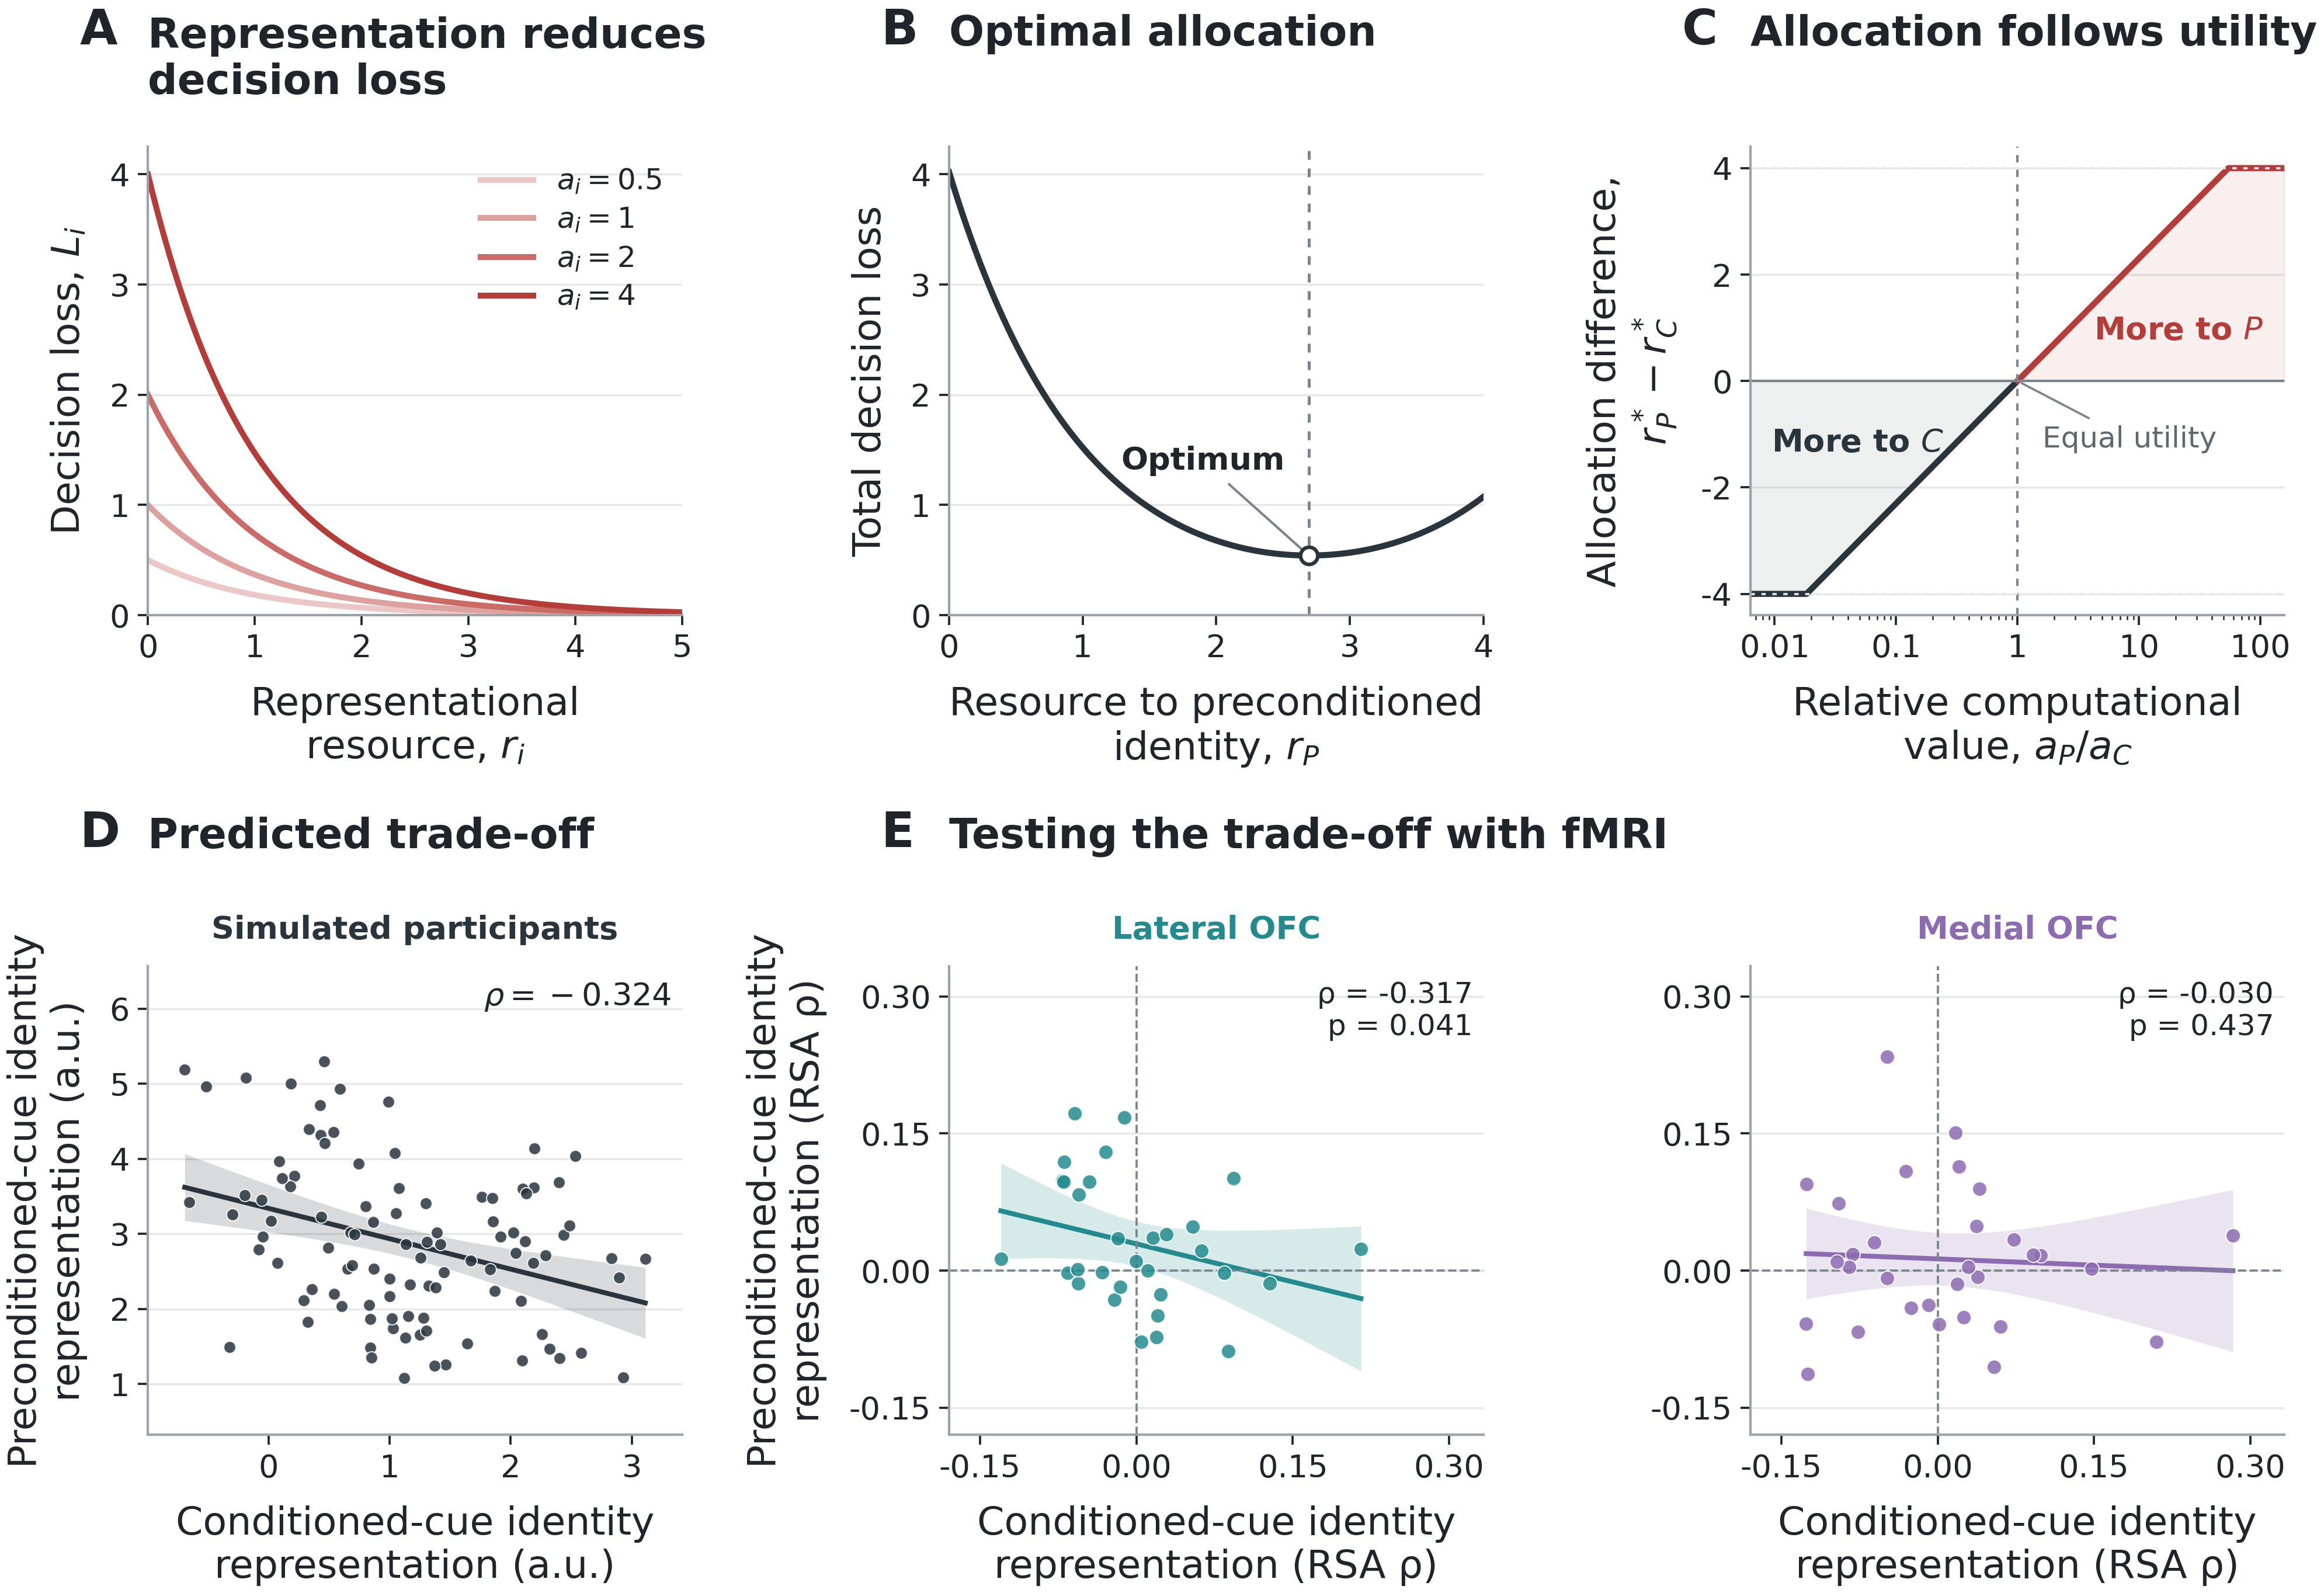
\includegraphics[width=0.95\linewidth]{../../fig/fig5_model.png}
\end{center}
\par\noindent\textbf{Figure~\thefigure. }
\textbf{A resource-limited model of outcome-identity representation.}
\textbf{A. Representation reduces decision loss.} Decision loss for cue $i$ decreases as representational resource $r_i$ is allocated to its outcome representation, according to $L_i=a_i e^{-r_i}$. Larger values of $a_i$ indicate a greater computational cost of weak outcome representations, while the exponential form produces diminishing returns.
\textbf{B. Optimal allocation.} When expectations based on preconditioned cues ($P$) and conditioned cues ($C$) share a finite representational budget, $r_P+r_C=R$, total decision loss is minimized by allocating resources according to their relative computational value. For the illustrative parameters $R=4$, $a_P=4$, and $a_C=1$, the optimum is $r_P^*=2.69$ and $r_C^*=1.31$.
\textbf{C. Allocation follows utility.} The optimal allocation difference is $r_P^*-r_C^*=\log(a_P/a_C)$ for interior solutions and is bounded by $\pm R$ because allocations must be nonnegative. Positive values indicate greater allocation to preconditioned cues ($P$), and negative values indicate greater allocation to conditioned cues ($C$). Thus, preferential representation of inferred outcomes emerges when their explicit representation has greater computational value ($a_P>a_C$); it is not imposed by cue category. The curve shows the general allocation rule; panel D restricts simulated parameters to the task-specific case $a_P>a_C$.
\textbf{D. Predicted trade-off.} A shared budget held constant across simulated participants predicts a negative relationship between direct and inferred identity representations. For 100 participants, $\log(a_P/a_C)$ was sampled from a normal distribution with underlying mean $\log 4$ and standard deviation $1.2$, truncated to positive values to enforce $a_P>a_C$. Independent Gaussian measurement noise (standard deviation $0.75$) was added to each optimal allocation. Points show simulated representational strengths in arbitrary units, yielding Spearman $\rho=-0.324$. Parameters are illustrative and were not fitted to the fMRI data; full sampling details are given in Supplementary Methods.
\textbf{E. Testing the trade-off in fMRI data.} Participant-level odor-identity RSA coefficients for conditioned and preconditioned cues were correlated across participants within lateral OFC (teal) and medial OFC (purple; $n=31$ for each region). The correlation was negative in lateral OFC (Spearman $\rho=-0.317$, $p=0.041$) and not significant in medial OFC ($\rho=-0.030$, $p=0.437$); $p$ values are from one-sided tests of predicted negative correlation. Dashed lines indicate zero RSA coefficients. In D and E, solid lines show descriptive linear least-squares fits, and shading indicates pointwise 95\% confidence intervals for the fitted mean response.
\par

\label{fig-identity-simu}

\par\endgroup\bigskip





\section*{Discussion}



\subsection*{Information content of inferred outcomes}

Our behavioral findings show that model-based inference in sensory preconditioning extends beyond the retrieval of scalar reward value to include information about specific outcome identity. Selective satiation reduced choices not only for directly conditioned cues associated with the devalued odor, but also for preconditioned cues that had never been directly paired with that odor. Because the value of the visual cues themselves was never directly updated after satiation, this transfer of devaluation to preconditioned cues requires access to information about the specific outcome predicted through the learned associative chain. These findings extend previous evidence that responding to preconditioned cues is sensitive to reinforcer devaluation in rodents \citep{hart20} and complement human work showing that OFC activity during sensory preconditioning contains information about inferred outcomes \citep{wang2020interactions}.


\subsection*{Representational nature of inferred rewards}

Our cross-task decoding results further suggest that inferred outcome expectations involve reactivation of experienced outcomes. A classifier trained to distinguish smelling different food odors in an independent localizer task successfully identified the inferred odor identity from lateral OFC responses to preconditioned cues, even though no odors were delivered during the probe test. Previous studies have shown that anticipation and receipt of reward value evoke similar neural representations in the OFC \citep{RN1}, and that this similarity develops as cue--outcome associations are learned \citep{kahnt2011decoding}. Our findings extend this account to specific outcome identities inferred through separately learned associations. Because preconditioned cues had never been directly paired with the odors, these results suggest that associative inference can reinstate representations of outcomes that have not been directly associated with the current cue.


\subsection*{Adaptive representation of reward identity in lateral OFC}

Our neural findings further suggest that reward-identity representations in lateral OFC are not expressed uniformly across all reward-predictive cues. Previous studies using directly learned cue--outcome associations have consistently identified identity-specific reward representations in lateral OFC, including representations that are updated by selective devaluation and predict subsequent goal-directed choices \citep{howard2015identity,howard2017identity,howard2018identity,liuyaoatt24,witkowski2026identity}. In the present task, however, identity information in lateral OFC was preferentially expressed for preconditioned cues, whose outcomes had to be inferred through an associative chain, rather than for conditioned cues whose outcome identities were directly learned. Thus, the present findings do not simply extend previous work by showing that lateral OFC represents another class of reward prediction. Instead, they suggest that the content of lateral OFC representations may depend on the computational demands imposed by the current task.

This interpretation is consistent with cognitive-map accounts proposing that OFC represents task-state information that is relevant but may not be directly observable for ongoing learning and decision making \citep{wilson2014orbitofrontal,schuck2016human,niv2019learning}. A central problem for such accounts is determining which of the many available features should be included in the task-state representation. Our resource-limited model provides one possible principle: detailed information about outcomes should be represented where doing so provides the greatest marginal computational benefit. Under a cost on representational resources, this difference can make explicit outcome-identity representations more valuable for preconditioned cues, producing the observed representational asymmetry without assuming that lateral OFC is intrinsically specialized for preconditioned cues.

A related principle has been proposed in sensory processing. Efficient-coding models predict that greater perceptual uncertainty increases the neural resources devoted to stimulus encoding \citep{mlynarski2022efficient}, and task-related enhancement of category information in inferotemporal cortex is greater for more ambiguous stimuli \citep{dehaqani2022neural}. Our model applies a similar allocation principle to outcome identity, proposing that explicit representations receive more resources when errors in recovering that identity are more likely or more costly.

More broadly, this account is compatible with prior work showing that working-memory constraints shape reinforcement learning, such that learning performance declines as the number of stimulus–response associations increases \citep{collins2012much,collins2018tortoise}. In our task, maintaining outcome information for both conditioned and preconditioned cues may impose a conceptually similar competition for limited representational resources.


\subsection*{Limitation and future directions}

One limitation of our work is that the proposed resource-limited account is a normative but \textit{post-hoc} explanation of the observed representational asymmetry rather than an \textit{a priori} model that the present experiment was designed to test. In particular, the behavioral cost of failing to recover the correct outcome identity, \(D_i\), was not experimentally varied and therefore remained effectively constant across conditions. Future studies could manipulate the consequences of errors, as well as the probability of outcome-identity retrieval errors, to test whether representational resources shift in the manner predicted by the model. Such manipulations would provide a more direct test of whether lateral OFC representations are allocated according to the computational utility of explicit outcome information.


A second limitation is the modest sample size. Thus, the nonsignificant findings for conditioned cues should not be interpreted as evidence that lateral OFC represents only preconditioned cues.


\subsection*{Conclusions}

Together, our findings show that model-based inference in sensory preconditioning extends beyond scalar reward value to include the identity of specific expected outcomes. Selective devaluation altered choices for both directly conditioned and preconditioned cues, demonstrating that behavior toward indirectly related cues depends on access to specific outcome information. At the neural level, lateral OFC represented expected outcome identity for preconditioned cues and these anticipatory representations overlap with those of experienced rewards. These effects were not significant for conditioned cues. Our resource-limited model provides a possible framework for understanding how the computational benefit of outcome information could guide the allocation of representational resources. More broadly, these findings support the view of OFC as an adaptive cognitive map whose representational content is shaped by the information most useful for current behavior.





\section*{Materials and methods}


\subsection*{Study participants}

Thirty-five healthy, right-handed adults provided written informed consent; 34 completed all sessions. Two were excluded for consistently poor conditioning accuracy ($<0.40$) and one for a persistent preference for clean-air cues and absent odor devaluation. The final sample comprised 31 participants (20 females; ages 21--42 years, $M = 28.58$, $SD = 6.03$). Odor pleasantness, hunger, and satiety ratings were unavailable for one participant ($n = 30$ for rating-based analyses). The NIDA-IRP Institutional Review Board approved the protocol (Study~\#001156), which was registered on ClinicalTrials.gov (NCT05707806).

\subsection*{Experimental design}

We combined sensory preconditioning with selective outcome devaluation (\autoref{fig-design}). An initial session selected visual cues with similar liking ratings and two pleasant, similarly preferred food odors (one sweet, one savory). On Day~1, participants completed fMRI localizers before associative learning and then learned six visual cue pairs across two stimulus sets (A1--B1, A2--B2, and C--D in each set). On Day~2, a preconditioning refresher was followed by three conditioning runs in which B1 and B2 predicted the two food odors and D predicted clean air. Participants then completed three probe runs each before and after a meal matching the B2-associated odor. Probe trials presented two conditioned or two preconditioned cues sequentially; participants chose the cue associated with their preferred outcome without receiving odors during the task. Odor pleasantness, hunger, and satiety were rated before and after the meal. Visual cue categories and sweet/savory assignments were counterbalanced across participants. Detailed task procedures, meal consumption, MRI acquisition, and preprocessing are described in Supplementary Methods.

\subsection*{Task stimuli}

Visual cues were grayscale cartoon characters and places selected to minimize preexisting preferences. Participant-specific sweet and savory food odors were delivered with a computer-controlled olfactometer that maintained constant airflow; clean air served as the control outcome. Stimulus selection and delivery specifications are provided in Supplementary Methods.

\subsection*{Behavioral data analysis}

Learning was quantified by run-wise accuracy, and Friedman tests compared performance across cue types. Probe choices were summarized as pairwise choice proportions, pooling valid trials across runs and stimulus sets. Two-sided Wilcoxon signed-rank tests assessed pre- to post-meal changes in choices and odor pleasantness. To test selective devaluation, one-sided Wilcoxon signed-rank tests compared changes for the devalued and non-devalued odors and, separately, changes in choices of their associated cues over clean-air cues within each cue class. These tests assessed whether the devalued condition showed a greater decrease. Behavioral tests used an uncorrected threshold of $p < 0.05$; detailed trial-inclusion rules are provided in Supplementary Methods.

\subsection*{Single-presentation GLMs}

To obtain multivoxel activity patterns for the representational analyses, we estimated separate beta patterns for individual probe cue presentations and odor-localizer trials using least-squares-separate general linear models (GLMs) \citep{mumford2012deconvolving}. Each probe model included a regressor for the target cue presentation (3\,s duration) and a second regressor pooling all other cue presentations within the run. Both cue positions were estimated. Models additionally included decision periods, left- and right-hand button presses, and motion, respiratory, and image-artifact nuisance regressors. Odor-localizer models similarly separated each target presentation from the remaining presentations, with events modeled at sniff-cue onset. Models used a 128\,s high-pass filter. Full model and nuisance-regressor specifications are provided in Supplementary Methods.

\subsection*{Region-of-interest definition}

The RSA and cross-task decoding used the same two independently defined bilateral orbitofrontal cortex (OFC) regions from a connectivity-based parcellation \citep{kahnt2012connectivity}: medial/posterior-lateral OFC (hereafter medial OFC) and central/anterior-lateral OFC (hereafter lateral OFC). Masks were resampled to the 2\,mm isotropic analysis grid and intersected with an SPM12 gray-matter mask (probability $>0.1$).

\subsection*{Representational similarity analysis}
\label{rsa-probe}

We used RSA to test whether cues predicting the same odor evoked more similar fMRI activity patterns than cues predicting different odors. To avoid any contamination between representations evoked by the first and second cue in each trial as well as changes in outcome value from pre- to post-meal, analyses focused on data from the first cue in each pre-meal probe trial, before devaluation could alter outcome value. Conditioned and preconditioned cues were analyzed separately, each comprising four odor-predictive images across the two stimulus sets; clean-air cues were excluded. Individual presentation patterns were retained without averaging across trials or runs.

Within each ROI and cue class, voxel responses were mean-centered across presentations within each run. Neural representational dissimilarity matrices (RDMs) were computed as one minus the Pearson correlation between presentation patterns. An odor-identity model RDM assigned zero to pairs predicting the same odor and one to pairs predicting different odors. We related the neural and model RDMs using Spearman correlation, retaining only comparisons between presentations acquired in different runs. Positive coefficients therefore indicate that neural patterns were more similar for cues associated with the same odor. One-sided one-sample t tests assessed participant-level coefficients against zero. To test the predicted trade-off between directly learned and inferred identity representations, we also correlated conditioned- and preconditioned-cue coefficients across participants within each ROI using one-sided Spearman tests of negative association ($p < 0.05$, uncorrected).

\subsection*{Cross-task decoding of odor identity}

We tested whether representations evoked by experienced odors generalized to visual cues predicting those odors. For each participant and ROI, a linear support vector machine with a fixed regularization parameter ($C = 1$) was trained to distinguish the two food odors using beta patterns from the passive odor localizer conducted before associative learning. Training included 40 presentations across two runs (20 per odor). The trained classifier was then applied to first-cue patterns from the pre-meal probe, during which no odors were delivered. Conditioned and preconditioned cues were tested separately, with cue labels indicating their associated odor; clean-air trials were excluded from training and testing.

Voxel responses were z-scored across presentations independently within each run and task. The classifier was trained on both odor-localizer runs and applied to probe patterns without further fitting or hyperparameter selection. Accuracy was averaged across the two odor identities, and one-sided one-sample t tests assessed whether participant-level accuracy exceeded 50\%. Successful transfer would indicate correspondence between the patterns elicited by perceived odors and those elicited by their associated visual cues, including cues whose outcomes must be inferred through the learned associations.

\subsection*{Searchlight RSA of subjective odor value}

To identify representations related to current outcome value, we performed searchlight multiple-regression RSA combining pre-meal and post-meal probe patterns ($n = 30$). Analyses included all cues and outcome types, including clean air. Pleasantness ratings were jointly standardized across phases, and each presentation was assigned the rating of its associated outcome in the corresponding phase. The value model RDM contained absolute differences between these ratings. Neural dissimilarities (one minus Pearson correlation) were regressed on the value RDM together with cue type, image identity, button presence, and button side RDMs. Only between-run pairs were retained, including comparisons across probe phases.

Participant-level value-coefficient maps were smoothed with a 6\,mm FWHM kernel and tested against zero using one-sided one-sample t tests in SPM12. Peak-level inference controlled family-wise error at $p < 0.05$ separately within the independently defined medial and lateral OFC masks \citep{kahnt2012connectivity}. Full model specifications and mask definitions are provided in Supplementary Methods.






\section*{Data availability}
De-identified behavioral data as well as analysis and simulation code are available at https://github.com/QingfangLiu/project-spcd. Additional data are available from the corresponding author upon reasonable request, subject to applicable institutional and participant-consent restrictions.




\section*{Acknowledgments}
This work was supported by the Intramural Research Program at the National Institute on Drug Abuse (ZIA DA000642 to T.K. and DA000587 to G.S.), as well as by a fellowship from the National Institutes of Health (NIH) Center on Compulsive Behaviors (to Q.L.). The contributions of the NIH authors are considered “works of the United States government.” The findings and conclusions presented in this paper are those of the authors and do not necessarily reflect the views of the NIH or the US Department of Health and Human Services.









\bibliographystyle{plainnat}
\bibliography{../main/sn-bibliography}

\end{document}
